This section outlines the categorization of signal events and the background estimation strategy for the \zh{} analysis. As noted in the introduction to this chapter, the \zh{} analysis is summarized only briefly, since the primary focus of this thesis is on the \wh{} channel. Nevertheless, the \zh{} channel represents an essential component of the full \vh{} measurement and therefore cannot be omitted.

The $\zh{} \to ZWW^{*} \to \ell\ell\ell\nu\ell\nu$ analysis requires the presence of exactly four isolated leptons (muons or electrons, including those from $\tau$ decays) with $\pt > 10$~GeV, a total lepton charge of zero, and at least one lepton matched to the trigger object.

To reconstruct the \zh{} process, a lepton-labeling scheme is employed to identify which leptons originate from the associated $Z$ boson and which from the Higgs boson. The leptons from the $Z$ boson are assigned first by selecting the SFOS lepton pair whose invariant mass is closest to the $Z$ boson mass. These leptons are labeled as \ltwo{} and \lthree{}, with the ordering $\pt(\ltwo) > \pt(\lthree)$. The remaining two leptons are then associated with the Higgs boson and labeled as \lzero{} and \lone{}, again ordered by transverse momentum such that $\pt(\lzero) > \pt(\lone)$. Figure~\ref{fig:zh_feynmann} illustrates this lepton-labeling scheme for this channel.

\begin{figure}
  \centering
  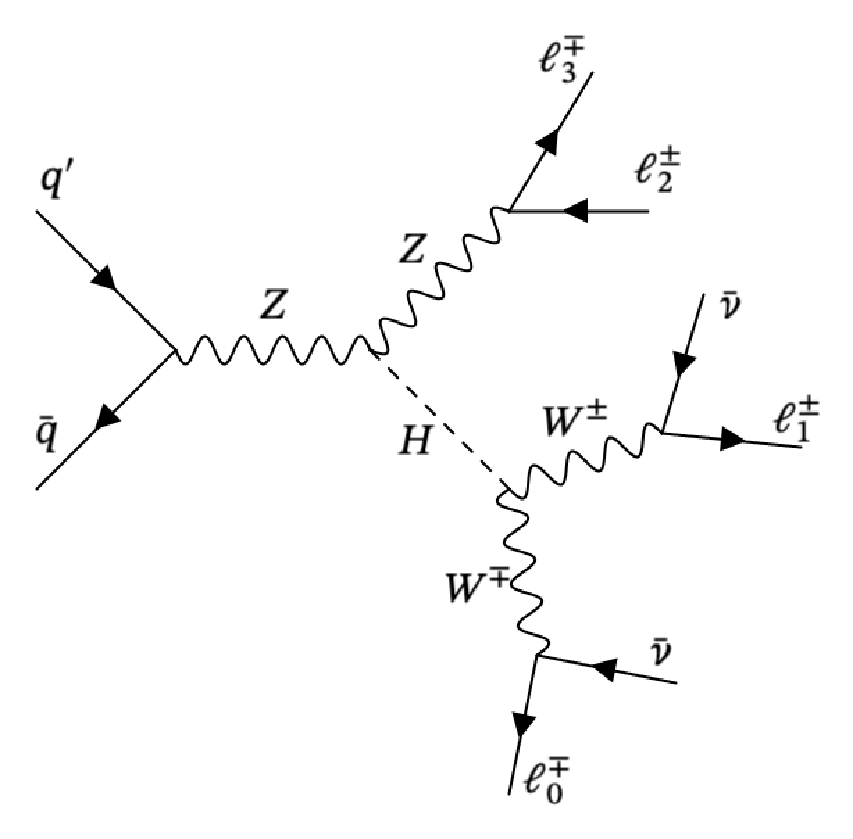
\includegraphics[width=0.5\linewidth]{figures/VH/VH_zh_feynmann.pdf}
  \caption{Lepton labeling scheme for the \zh{} analysis. The leptons from the $Z$ boson are labeled as \ltwo{} and \lthree{}, while those from the Higgs boson are labeled as \lzero{} and \lone{}.}\label{fig:zh_feynmann}
\end{figure}

Backgrounds in this channel are estimated following a strategy similar to that used in the \wh{} analysis. Many processes are modeled using MC simulation, while dominant contributions such as $ZZ^{*}$ are estimated using a hybrid data-MC approach. In this method, normalization factors are derived in control regions enriched in the relevant background. Contributions from fake leptons, originating from processes such as $Z+$jets and $t\bar{t}$, are estimated using a data-driven fake-factor method.

The $ZZ^{*} \to 4\ell$ process constitutes the largest background in the \zh{} analysis. Since $\tau$ leptons are not directly reconstructed, final states may consist not only of two SFOS pairs but also of one SFOS pair and one different-flavor opposite-sign (DFOS) pair. To account for this, and following the strategy applied in the \wh{} analysis, events are categorized by the number of SFOS pairs they contain. This classification enhances the sensitivity of the measurement, particularly by targeting the two-SFOS-pair region, where the $ZZ^{*}$ background is most prominent.

Dedicated ANNs are used in this analysis the enhance sensitivity with respect to a purely cut-based analysis. The one SFOS and two SFOS categories have different ANNs which are optimized for their respective background composition.